\documentclass[crop,tikz,border=10]{standalone}

\usepackage{amsmath, amssymb}
\usetikzlibrary{calc}

\begin{document}
    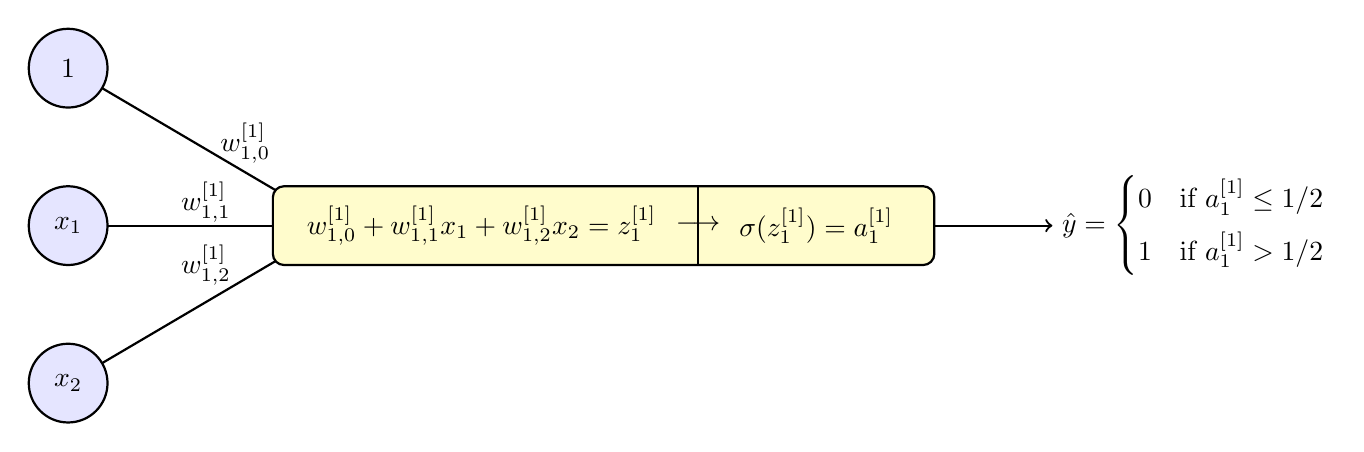
\begin{tikzpicture}
        \draw[thick] (-8, 2) -- (-4.6, 0);
        \draw[thick] (-8, 0) -- (-5, 0);
        \draw[thick] (-8, -2) -- (-4.6, 0);

        \node at (-5.75, 1.05) {$w^{[1]}_{1, 0}$};
        \node at (-6.25, 0.3) {$w^{[1]}_{1, 1}$};
        \node at (-6.25, -0.5) {$w^{[1]}_{1, 2}$};

        \draw[thick, rounded corners, fill=yellow!20] (-5.4, -0.5) rectangle (3, 0.5);
        \draw[thick] (0, -0.5) -- (0, 0.5);
        \node at (-2.75, 0) {$w_{1, 0}^{[1]} + w_{1, 1}^{[1]}x_1 + w_{1, 2}^{[1]}x_2 = z^{[1]}_1$};
        \node at (1.5, 0) {$\sigma(z_1^{[1]}) = a_1^{[1]}$};
        \node at (0, 0) {$\longrightarrow$};
        \draw[thick, ->] (3, 0) -- (4.5, 0);

        \draw[thick, fill=blue!10] (-8, 2) node {$1$} circle (0.5);
        \draw[thick, fill=blue!10] (-8, 0) node {$x_1$} circle (0.5);
        \draw[thick, fill=blue!10] (-8, -2) node {$x_2$} circle (0.5);

        \node[right] at (4.5, 0) {$\hat y =\displaystyle{\begin{cases}0&\text{if $a_1^{[1]}\leq 1/2$}\\[1ex]1&\text{if $a_1^{[1]}> 1/2$}\end{cases}}$};
    \end{tikzpicture}
\end{document}